\chapter[Implémentation de la solution]{Implémentation de la solution}

\textit{La phase d'analyse a permis de définir les objectifs du programme et d'organiser la phase de codage. Ce chapitre détaille les étapes de programmation effectivement réalisées, ainsi que les difficultés et les modifications ayant été apportée à la solution initiale.}

\section{Gestionnaire de version et environnement de développement}

Avant de débuter la programmation, une étape d'organisation a été nécessaire avec le commanditaire. En effet, afin de communiquer facilement sur l'avancée du projet, un gestionnaire de version a été mis en place. Cela a permis d'enregistrer les évolutions du programme, de manière à pouvoir rappeler une version antérieure fonctionnelle à tout moment. \\

Le gestionnaire de version choisi est Git. Ce logiciel libre, distribué sous la licence GNU, est considéré comme l'état de l'art dans l'industrie. Une organisation \textit{<activeML>} a été créée pour gérer facilement les projets sur GitHub. Ce système m'a permis d'interagir directement avec mon commanditaire en cas de problèmes ou de questions. Cependant, n'ayant jamais utilisé cet outil, sa prise en main a été compliquée.\\

Afin de faciliter la manipulation des commandes de Git, j'ai utilisé le plugin Git sur Atom. Développé par GitHub, cet éditeur de texte libre est très modulable.

\section{Phases de programmation}

\textit{Cette section vise à détailler les fonctionnalités générales à implémenter et les solutions apportées lors de la programmation.}

\subsection{Interface graphique}

Comme défini lors de l'analyse, la méthode Modèle/Vue/Contrôleur (MVC) a été utilisée pour structurer le code. Ainsi, pour la partie \textit{Vue}, trois interfaces graphiques ont été définies : une interface principale, une interface de chargement, et une interface pour corriger la classification. Ces trois interfaces ont été réalisées avec la bibliothèque multi-plateforme Qt.\\

La première phase de programmation a consisté à finaliser l'organisation de ces interfaces. Pour cela, l'environnement de développement Qt Creator a été choisi afin de faciliter la mise en place des objets. Le code issu de ce traitement a été transcrit en Python grâce à l'utilitaire Pyuic5. Il a ensuite fallu écrire un module permettant d'ouvrir ces fenêtres, et qui correspond à la partie \textit{Contrôleur}. \\

Les principales difficultés rencontrées dans cette phase sont liées à la compréhension du code des interfaces. Dans le code principal, trois nouvelles classes ont été créées pour gérer les connexions entre les interfaces : \textit{LoaderWindow}, \textit{MainWindow}, \textit{CorrectionWindow}. Ces classes héritent des trois classes initiales, créées par Pyuic5.

\begin{figure}[!h]
	\begin{center}
		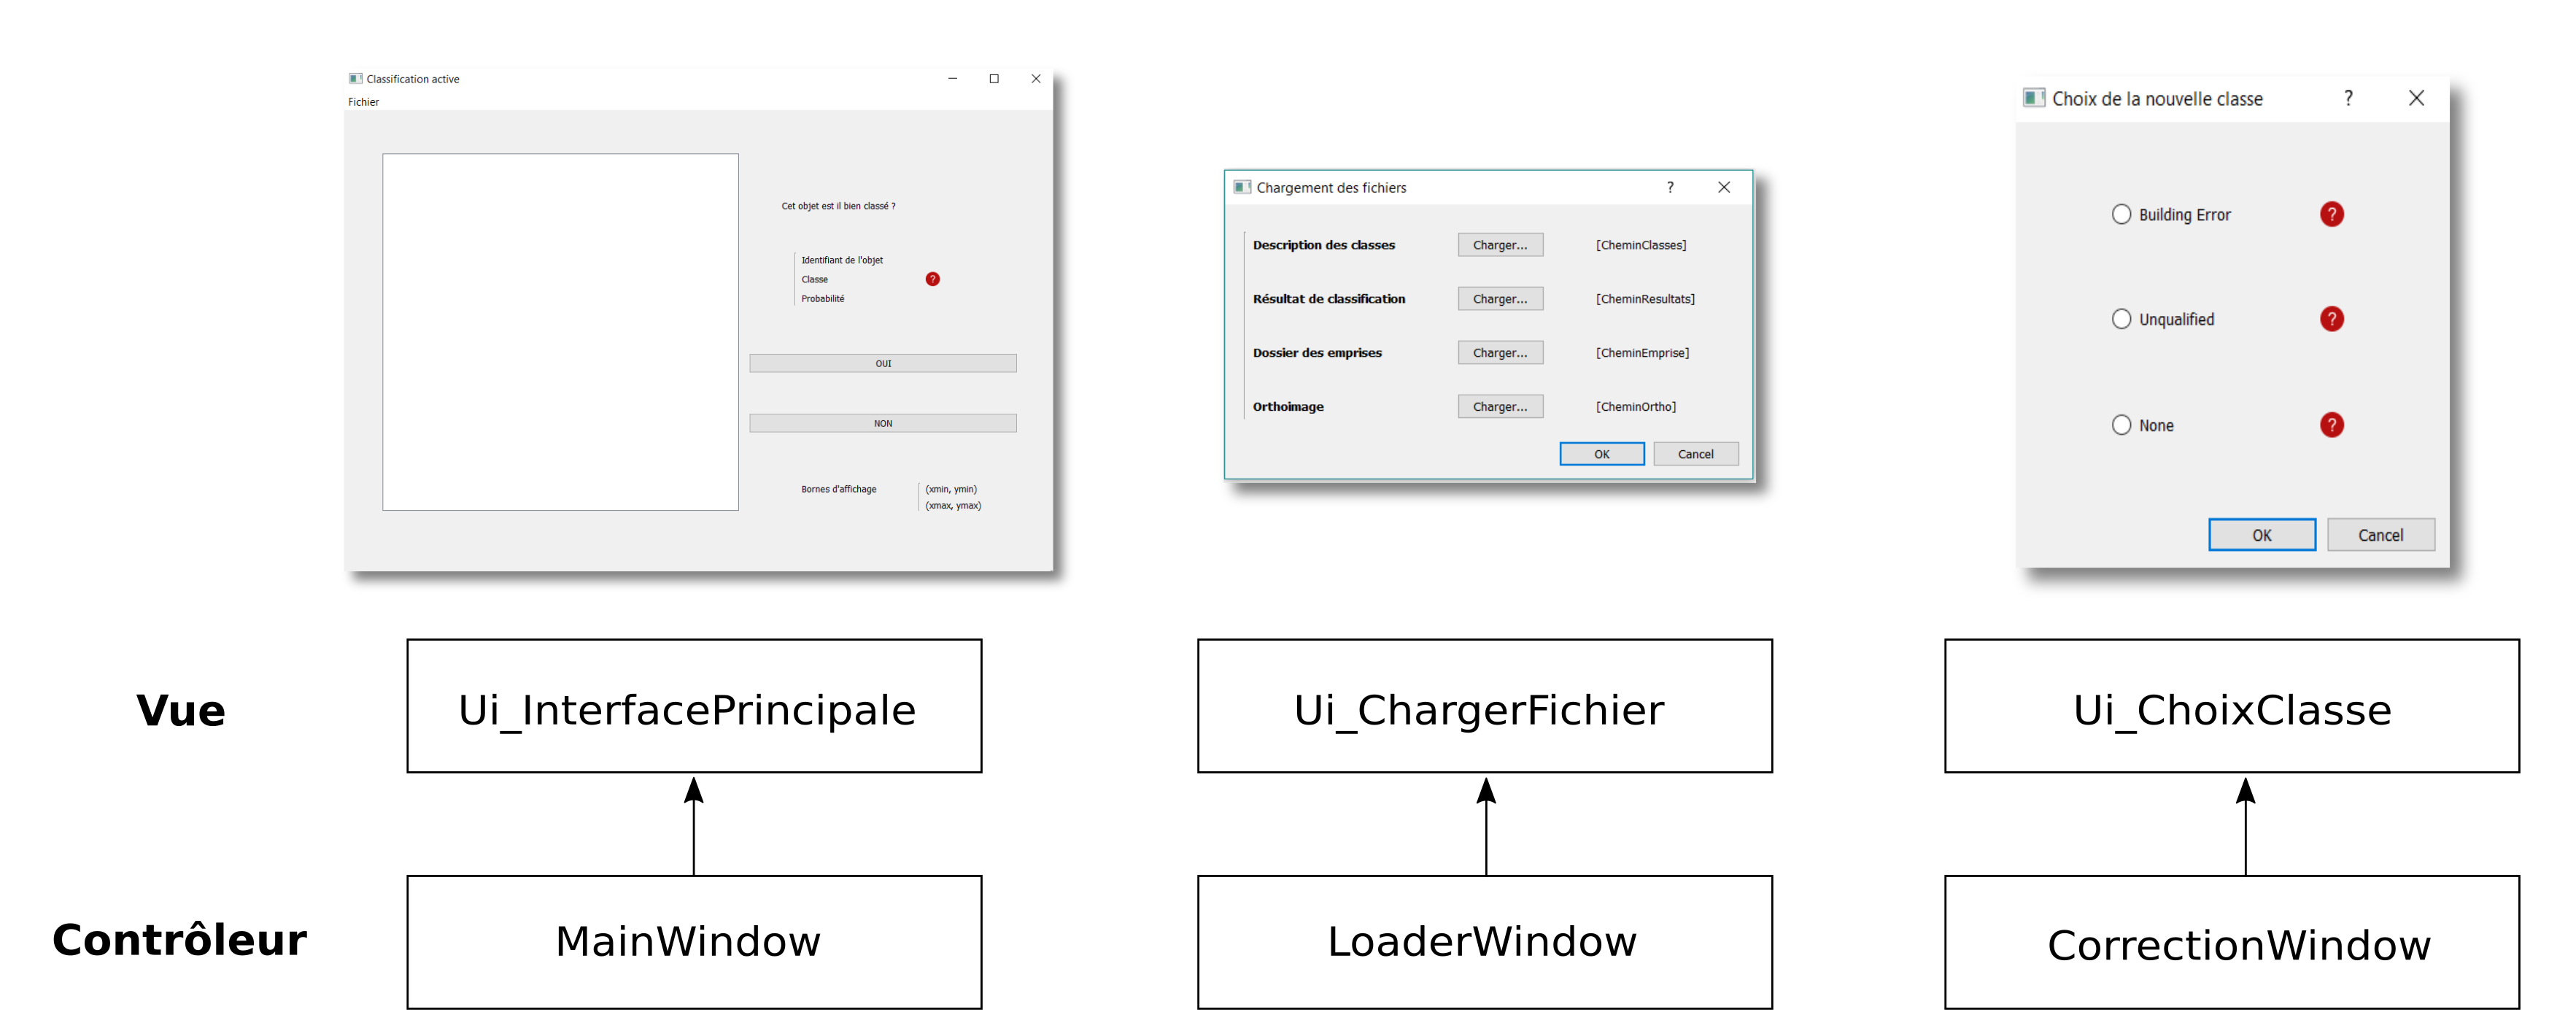
\includegraphics[scale=0.55]{Classes_interface.png}  
		\caption[Organisation des interfaces et héritages associés]{Organisation des interfaces et héritages associés}
		\label{fig:classeinterface}
	\end{center}
\end{figure}

\subsection{Chargement des données}

Pour permettre à l'utilisateur de charger les fichiers nécessaires au programme, une interface de chargement a été définie (\textit{LoaderWindow}). Elle permet de  sélectionner les 2 fichiers .CSV contenant les classes et les résultats de la qualification, le dossier contenant les emprises des entités et l'orthophoto associée. Cette interface de chargement est lancée en cliquant sur \textit{Fichiers > Charger...} , qui lance la fonction \textit{show\_loading\_window}.\\

\noindent Les difficultés rencontrées lors de la programmation sont de deux ordres :
\begin{itemize}[label=$\rightarrow$]
	\item L'établissement de la connexion entre le bouton et l'ouverture de la fenêtre de chargement : ce problème a été résolu par l'utilisation de la classe \textit{QFileDialog} de Qt. Ces connexions ont été implémentées dans la partie \textit{Contrôleur} du programme.
	\item L'enregistrement du chemin d'accès défini par l'utilisateur : après avoir réalisé des tests en créant une nouvelle classe \textit{Path}, le choix s'est finalement porté sur l'intégration d'un attribut à la classe \textit{LoaderWindow} pour chacun des chemins d'enregistrement.
\end{itemize}

Lorsque la phase de chargement est complétée, le programme principal peut s'exécuter. Comme prévu dans l'analyse, les caractéristiques des classes sont lues et enregistrées dans un dictionnaire, et les résultats de la qualification sont enregistrés dans une liste de tuples. L'orthoimage et les emprises ne sont lues que lors de l'affichage.

\subsection{Sélection des données}

Une fois l'étape de chargement des données effectuée, le programme en lui-même peut être lancé. Comme défini lors de l'analyse, l'étape suivante était de filtrer la liste des entités en entrée pour n'en présenter qu'un certain nombre à l'utilisateur. Cela s'apparente donc à la partie \textit{Modèle} du programme.\\

L'analyse préconisait la création d'une classe abstraite \textit{Strategy} permettant l'application du filtre. Les types de stratégies devaient être définies dans des classes qui  héritent de ces propriétés. Lors de la programmation, il est apparu que les classes abstraites en Python ne font pas parties du cœur même de Python, et sont accessibles grâce à la bibliothèque \textit{abc} (Abstract Base Classes). \\

\begin{figure}[!h]
	\begin{minipage}{0.50\linewidth}\parindent12pt
		\indent Pour simplifier la programmation, la classe mère \textit{Strategy} n'a pas été implémentée comme abstraite. Les classes filles héritent simplement des propriétés de la classe mère et viennent les compléter. \\\\
		\indent Dans un premier temps, seules les stratégies \textit{Naïve} (sélection de toutes les entités) et \textit{Random} (sélection d'un nombre aléatoire d'entités) ont été implémentées.
	\end{minipage}
	\hfill
	\begin{minipage}{0.45\linewidth}
		\centering
		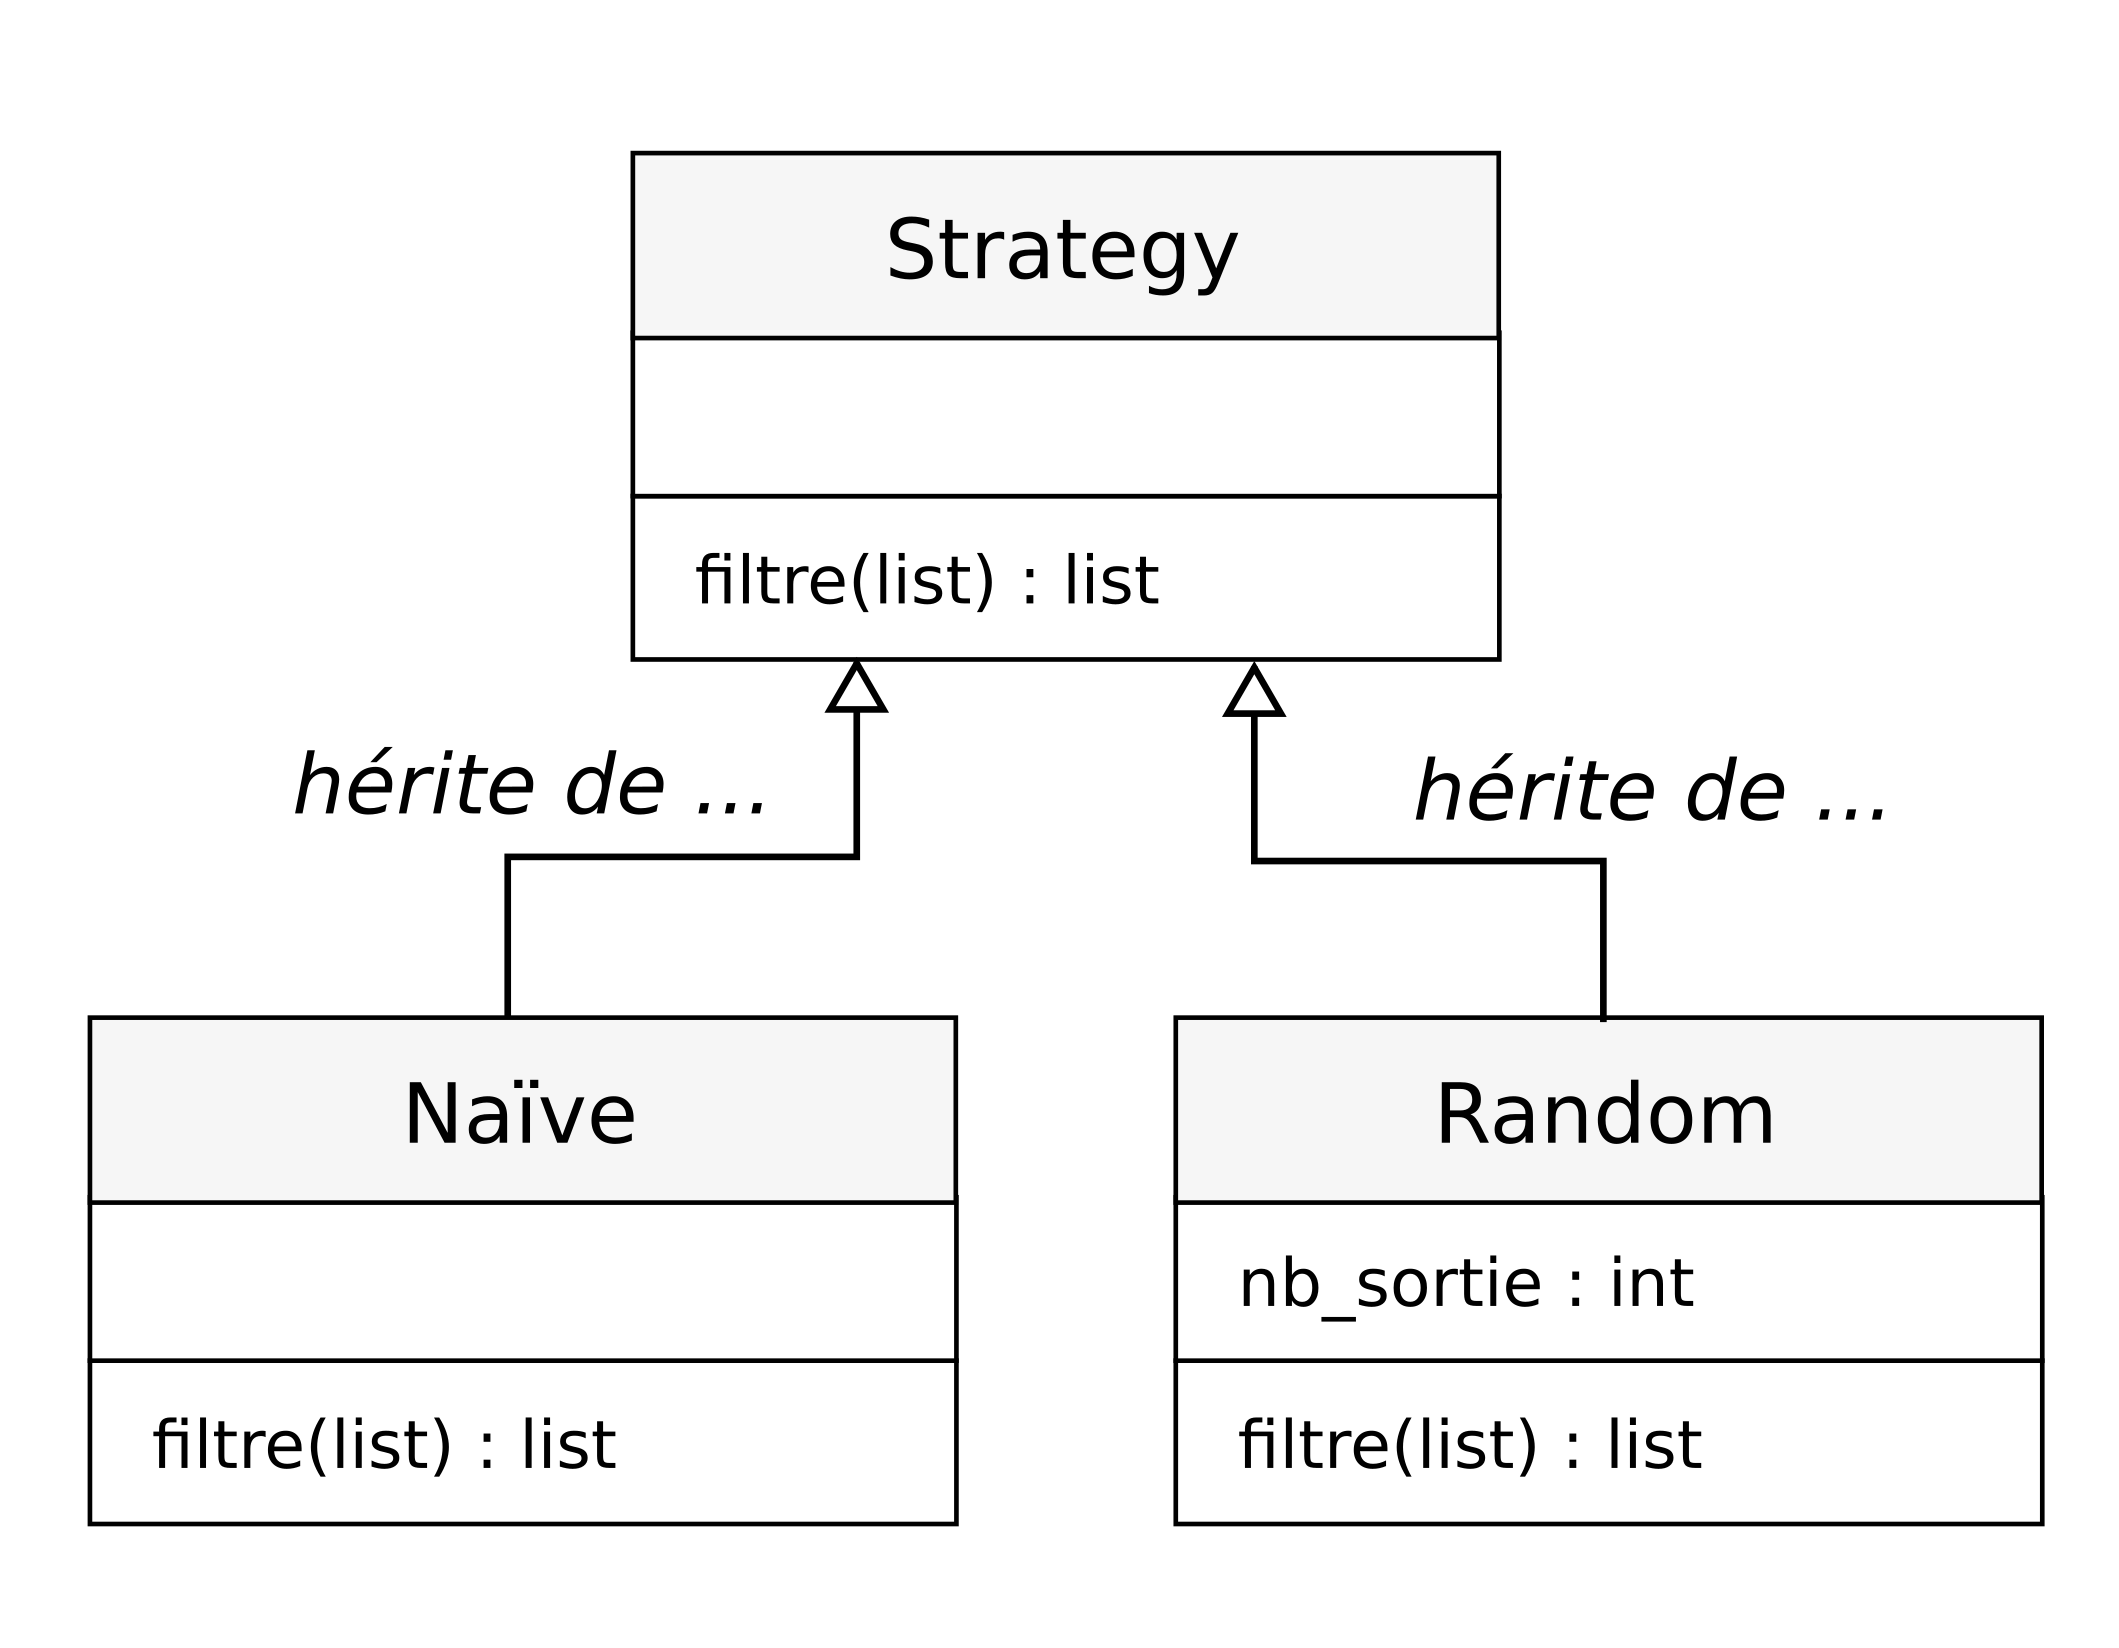
\includegraphics[scale=0.30]{classes_strategy.png}  \\
		\caption[Stratégies de sélection]{Stratégies de sélection}
		\label{fig:fonctionfiltre}
	\end{minipage}
\end{figure}

\begin{figure}[!h]
	\begin{minipage}{0.50\linewidth}\parindent12pt
		\indent  Une amélioration a été apportée au programme initialement imaginé. Elle permet à l'utilisateur de sélectionner la méthode de filtrage qu'il souhaite utiliser dans l'interface de chargement des fichiers. Pour ce faire, une variable globale \textit{STRATEGIES} regroupe, sous forme de dictionnaire, l'ensemble des classes filles de \textit{Strategy}. Cette variable est créée en utilisant la réflexion, c'est à dire en utilisant la capacité de Python à examiner ses propres structures internes.
	\end{minipage}
	\hfill
	\begin{minipage}{0.45\linewidth}
		\centering
		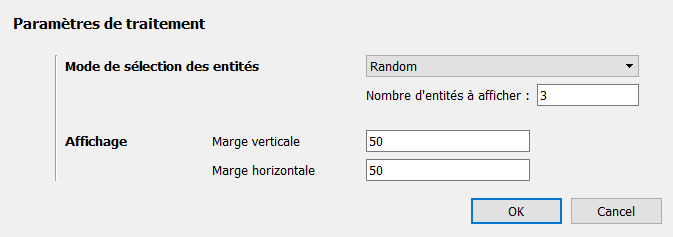
\includegraphics[scale=0.50]{interface_chargement_strategie.png}  \\
		\caption[Sélection de la stratégie dans l'interface de chargement]{Sélection de la stratégie dans l'interface de chargement}
		\label{fig:interfchargement}
	\end{minipage}
\end{figure}

\subsection{Visualisation des entités}

A ce point de la programmation, on obtient une liste de tuples correspondant aux objets à montrer à l'utilisateur. Lors de l'analyse, plusieurs étapes ont été définies pour afficher les différentes entités :
\begin{itemize}[label=$\rightarrow$]
	\item Création d'une liste d'objets \textit{Bâtiment} ;
	\item Calcul des limites d'affichage ;
	\item Préparation de l'affichage de l'orthoimage et des emprises ;
	\item Affichage des caractéristiques de l'entité.\\
\end{itemize}

\noindent On détaillera chacune de ces étapes et les problématiques qui lui sont liées.\\

\noindent\textbf{Création d'une liste d'objets \textit{Bâtiment}}\\

Une classe \textit{Building} a été créée pour enregistrer l'identifiant, la géométrie, la classe et la probabilité associée à chaque entité à afficher. Pour renseigner les attributs d'identifiant, de classe et de probabilité, on utilise simplement les valeurs du fichier des résultats de la classification.\\

\begin{figure}[!h]
	\begin{minipage}{0.55\linewidth}\parindent12pt
		\indent  Pour le renseignement de la géométrie des objets, l'implémentation a été plus compliquée. Les données de géométrie étaient initialement au format .GML. Cependant, la lecture de ces fichiers n'était pas gérée par le package \textit{gdal}. Les emprises au format .SHP ont donc été privilégiées. Pour lire la géométrie contenue dans ces fichiers, la fonction \textit{read\_building} a été implémentée. Elle se base sur les fonctions du package \textit{pyshp}.\\
	\end{minipage}
	\hfill
	\begin{minipage}{0.40\linewidth}
		\centering
		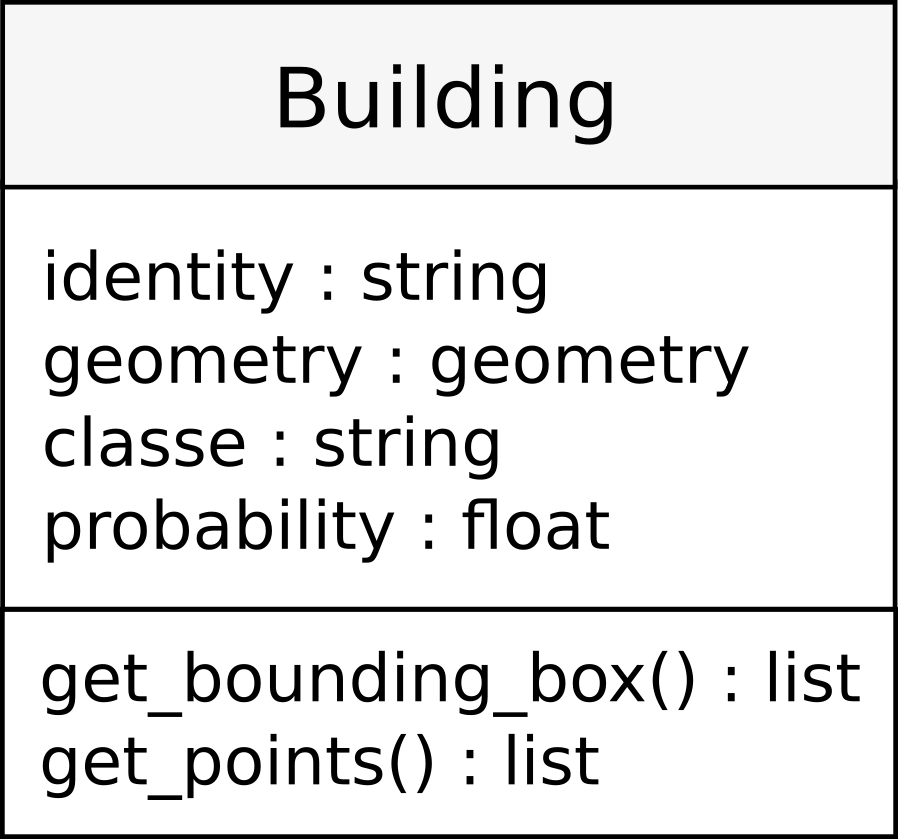
\includegraphics[scale=0.50]{building_classe.png}  \\
		\caption[Classe Building]{Classe Building}
		\label{fig:buildingclasse}
	\end{minipage}
\end{figure}

\newpage
\noindent\textbf{Calcul des limites d'affichage}\\
\begin{figure}[!h]
	\begin{minipage}{0.50\linewidth}\parindent12pt
		\indent  La détermination de la fenêtre d'affichage se base sur les coordonnées des extrémités des emprises. Pour les calculer, deux méthodes ont été créées dans la classe \textit{Building} : \textit{get\_points} qui récupère les points de la géométrie et \textit{get\_bounding\_box} qui sélectionne les maxima et minima. Lors de l'affichage, les marges entrées par l'utilisateur sont prises en compte. Un problème est apparu lorsque la marge dépasse l'image: une translation est donc réalisée.
	\end{minipage}
	\hfill
	\begin{minipage}{0.50\linewidth}
		\centering
		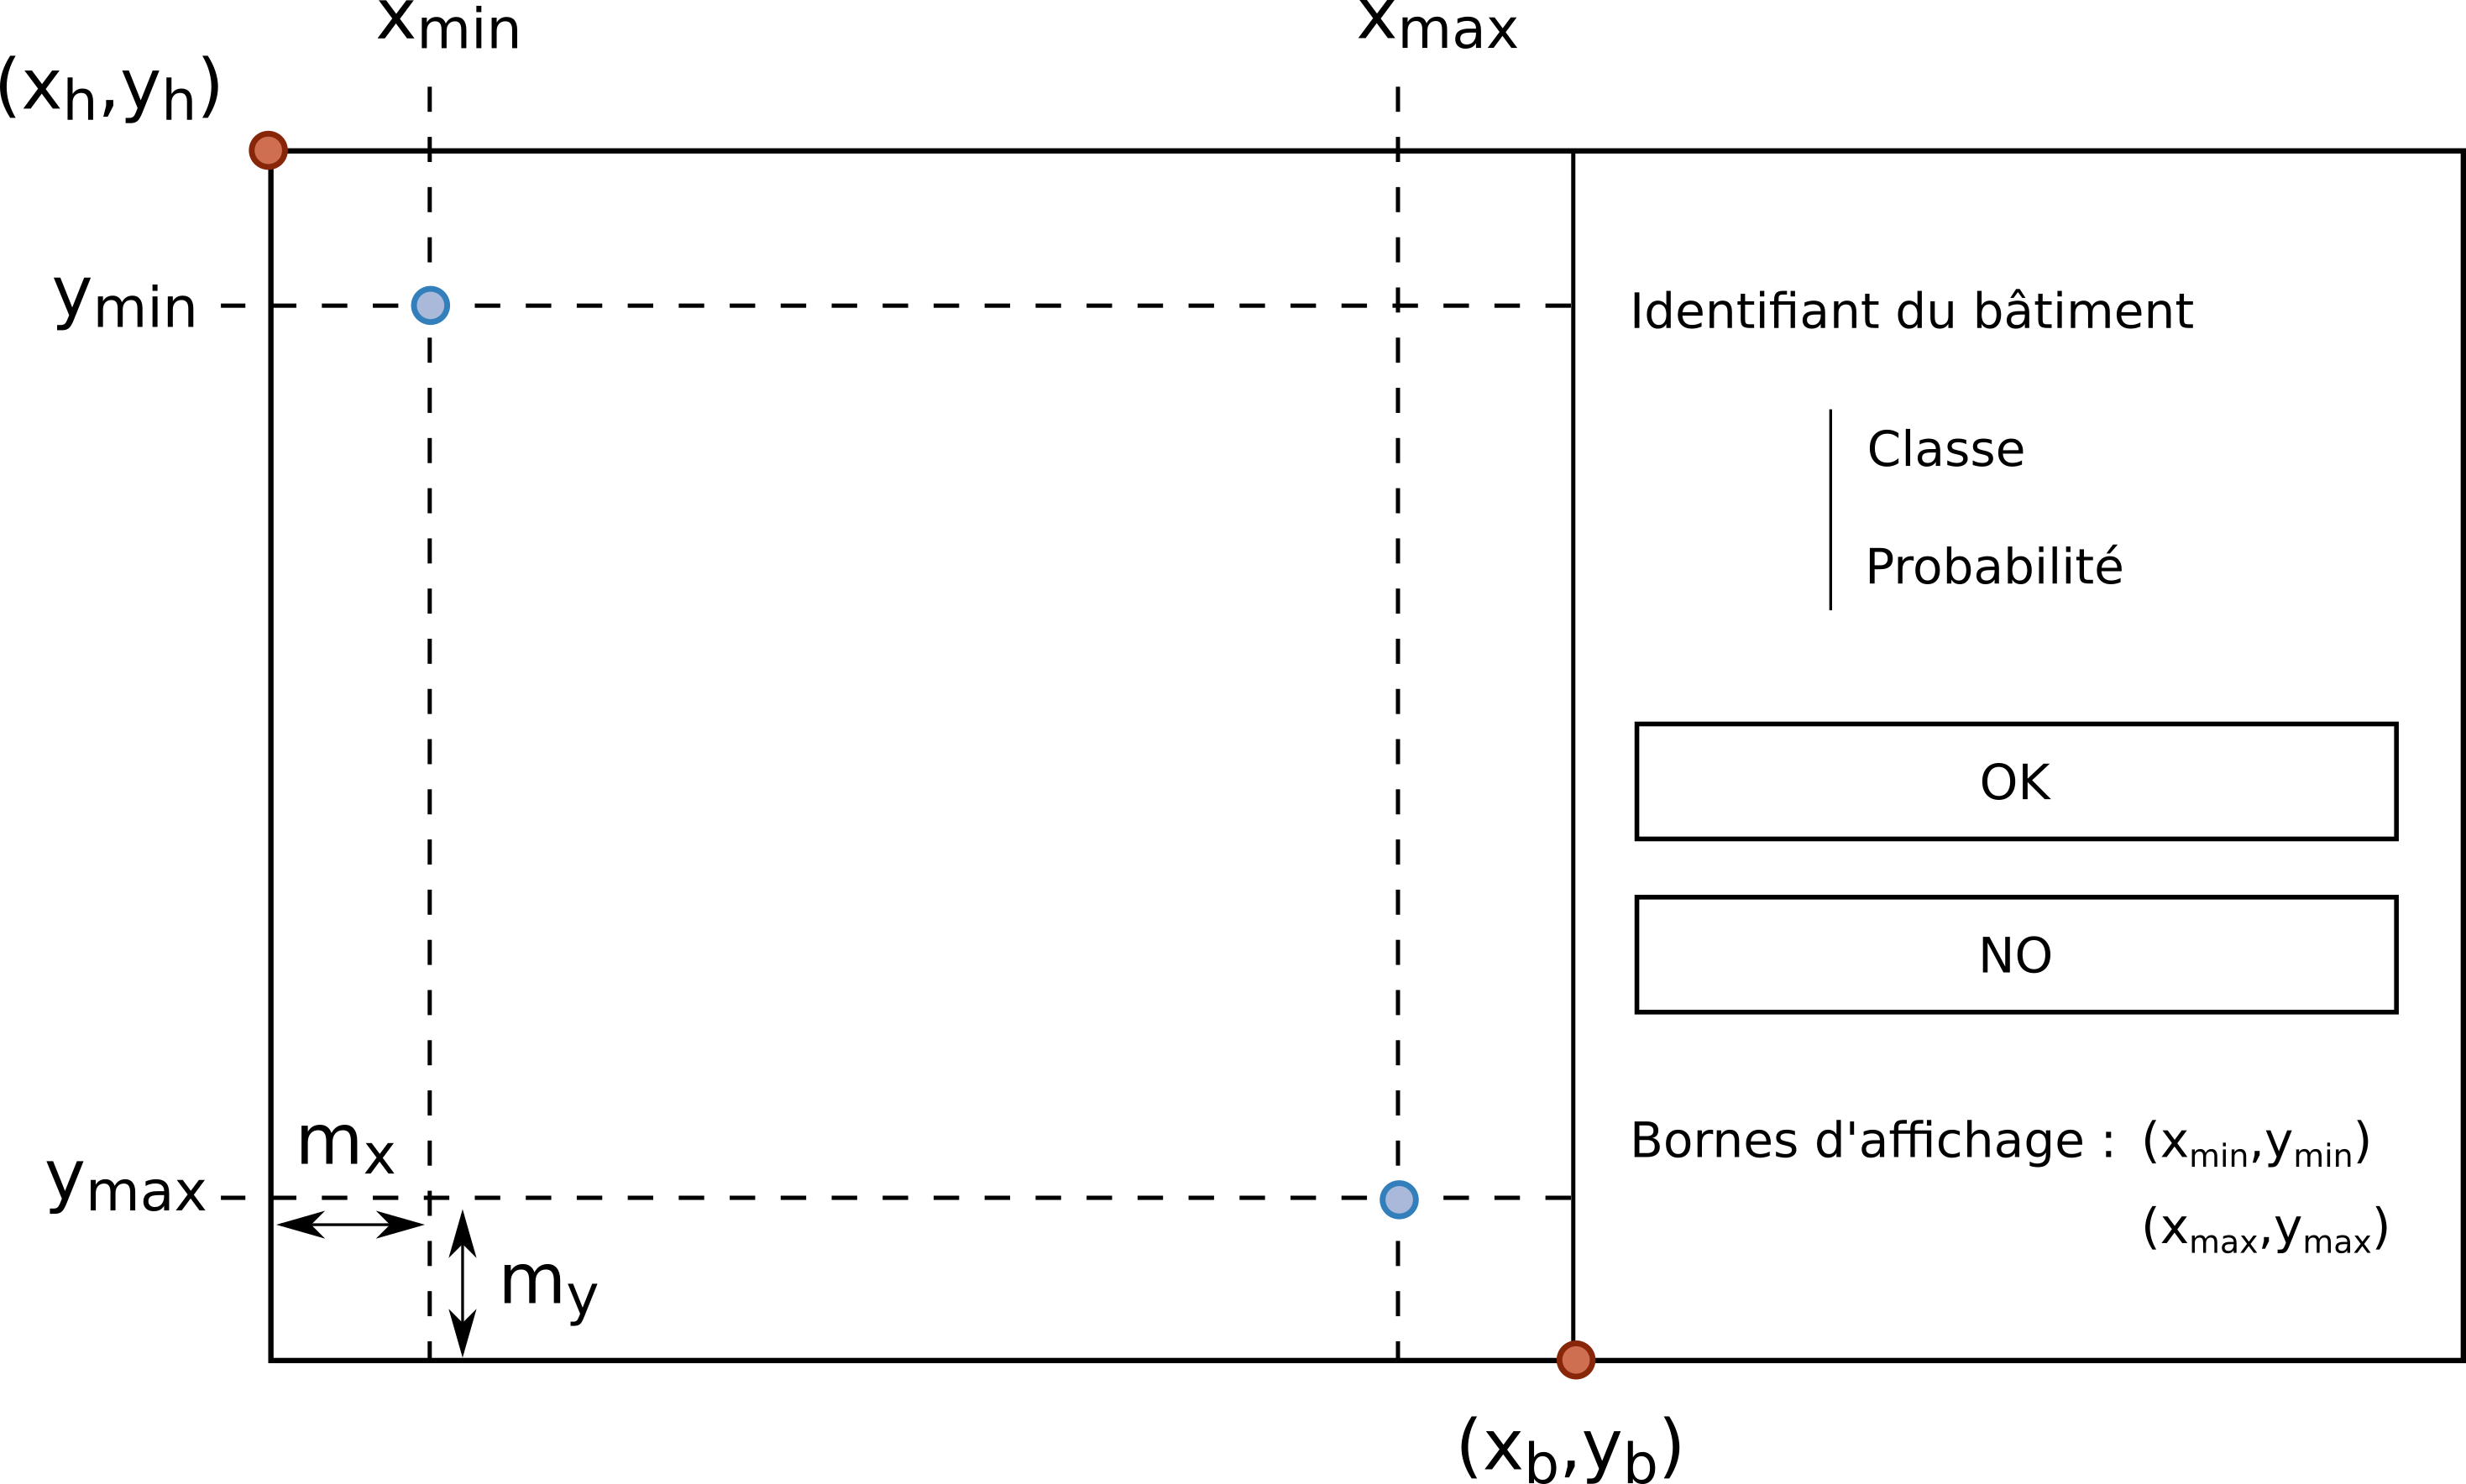
\includegraphics[scale=0.27]{interface_schema.png}  \\
		\caption[Limites d'affichage]{Limites d'affichage}
		\label{fig:interfschema}
	\end{minipage}
\end{figure}

\noindent\textbf{Affichage de l'orthoimage}\\

La lecture de l'orthoimage a nécessité plus d'étapes que prévues lors de l'analyse. Pour mieux organiser le code, une classe \textit{Background} a été créée. Elle prend comme attribut les coordonnées du point de référence de l'orthophoto, sa taille de pixel et la matrice d'image. Le package \textit{gdal} a été utilisé pour lire les données issues du fichier .TIFF.\\

\begin{figure}[!h]
	\begin{minipage}{0.50\linewidth}\parindent12pt
		\indent  Pour charger l'orthoimage et créer l'objet \textit{Background}, la fonction \textit{read\_background},  a été implémentée. Cette fonction est issue du programme  d'auto-qualification réalisé par Oussama ENNAFII, commanditaire du projet. Pour rogner l'orthoimage aux dimensions de l'entité, une méthode \textit{crop} a été ajoutée à la classe \textit{Background}. Elle retourne l'image couleur rognée.\\
	\end{minipage}
	\hfill
	\begin{minipage}{0.45\linewidth}
		\centering
		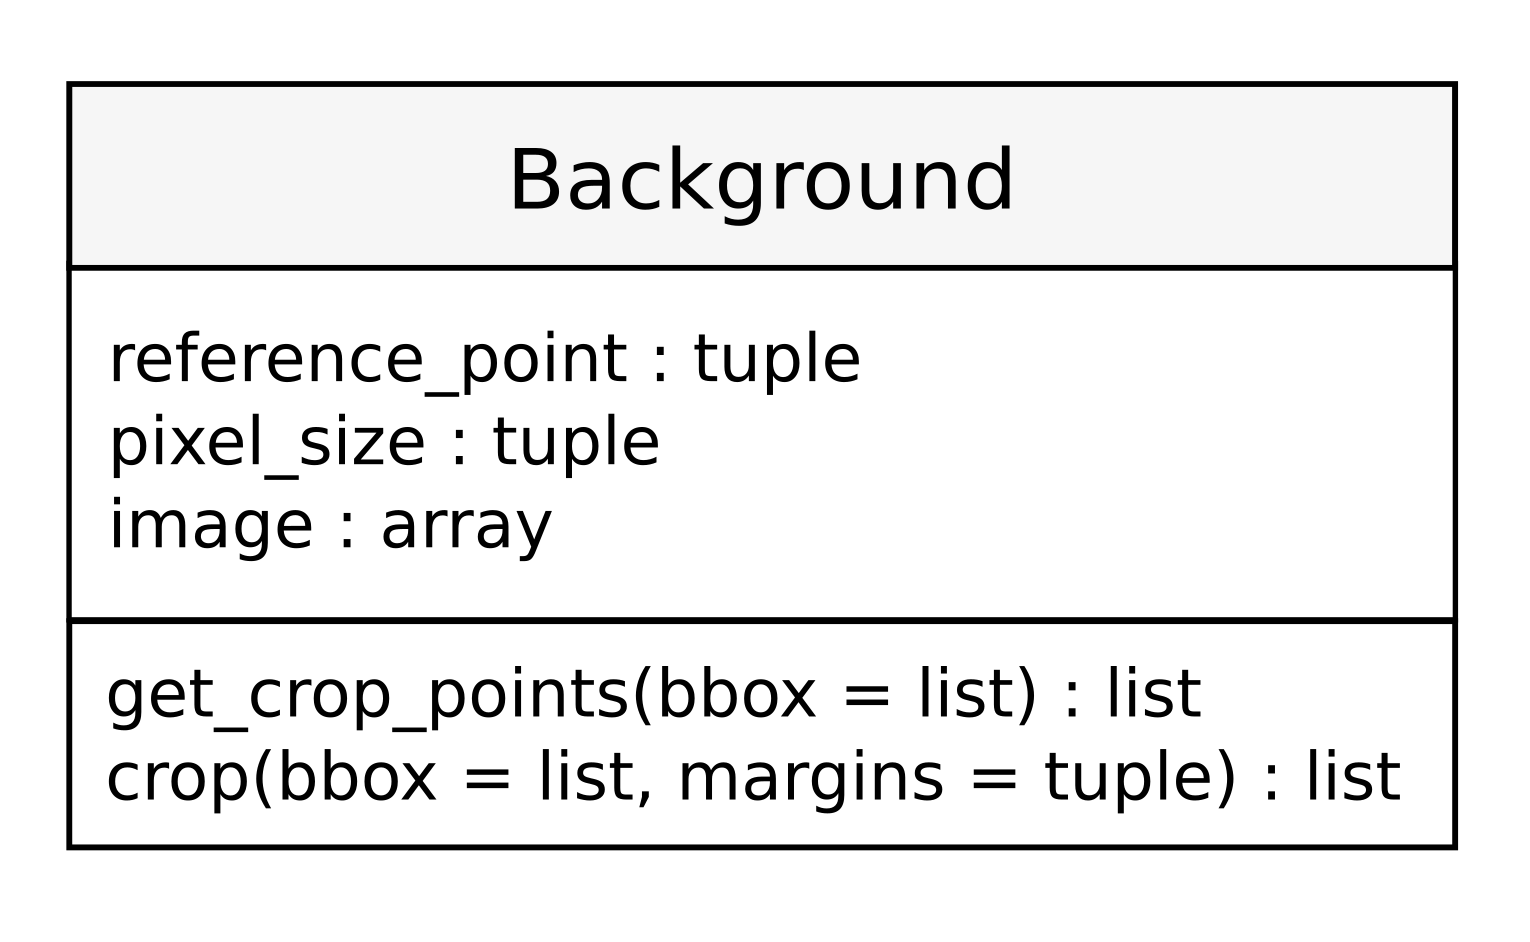
\includegraphics[scale=0.50]{background_classe.png}  \\
		\caption[Classe Background]{Classe Background}
		\label{fig:backclasse}
	\end{minipage}
\end{figure}

La phase d'affichage a nécessité l'utilisation des méthodes de l'objet \textit{QGraphicsView} de Qt. Des options particulières ont permis d'adapter la scène à la fenêtre graphique.\\

\noindent\textbf{Affichage des emprises}\\

L'affichage des géométries des entités a nécessité l'utilisation des méthodes des classes \textit{QPolygonF} et \textit{QPointF} de Qt. La principale difficulté a été de superposer l'entité à l'orthoimage en appliquant correctement les valeurs des marges.\\

\noindent\textbf{Affichage des caractéristiques de l'entité}\\

L'affichage des caractéristiques de l'entité est basée sur la lecture des attributs l'objet \textit{Building}. Des fonctionnalités supplémentaires ont été développées, comme l'affichage des coordonnées des bornes, ou l'inclusion d'infobulles expliquant le type de classe.

\newpage
\subsection{Interaction avec l'utilisateur}

Cette étape de la programmation correspond à la partie \textit{Contrôleur} du code. Grâce à l'affichage des entités et de leurs caractéristiques, l'utilisateur peut valider le résultat ou sélectionner une autre classe. \\

Initialement, une seule fonction était prévue pour cette phase d'interaction. Mais suite à des difficultés pour parcourir la liste des entités à présenter, un nouveau formalisme a été imaginé. Trois fonctions ont donc été créées :
\begin{itemize}[label=$\rightarrow$]
	\item La fonction \textit{next()} permet de parcourir la liste des entités à présenter et d'afficher son emprise et ses caractéristiques ;
	\item La fonction \textit{validate()} permet d'enregistrer l'entité présentée comme valide ;
	\item La fonction \textit{correct()} lance l'interface de sélection d'une nouvelle classe et enregistre le choix de l'utilisateur.\\
\end{itemize}

Lorsque la liste des entités à présenter est vide, la phase d'interaction avec l'utilisateur terminée. Une dernière fonction \textit{save()} est lancée. Elle permet de demander à l'utilisateur le chemin d'enregistrement des résultats. Si celui-ci n'est pas correctement défini, une fenêtre d'erreur s'affiche. Chaque entité visualisée est ensuite enregistrée dans un fichier .CSV, dont le formalisme est identique aux données en entrée. \\

\textit{Cette section a présenté les différentes étapes de programmation et les modifications apportées. En effet, la phase d'analyse avait permis de définir le cadre général du programme, mais son implémentation a mis à jour des difficultés non envisagées initialement.}\\

\section{Planning opérationnel}

Bien que plusieurs créneaux horaires aient été dédiés à la phase de programmation, le planning envisagé lors de la phase d'analyse n'a pas été complètement suivi. 

\begin{figure}[!h]
	\centering
	\includegraphics[scale=0.60]{planning_effectif.png}  \\
	\caption[Planning suivi pour la phase de programmation]{Planning suivi pour la phase de programmation}
	\label{fig:planning}
\end{figure}


